% vim: set tabstop=4 :

\newcommand{\figtb}[5]{ %引数 {日本語タイトル}{英語タイトル}{サイズ}{ファイル名}{ラベル名}
\begin{figure}[tb]
  \begin{center}
    \includegraphics[width=#3cm,clip]{figure/#4}
    \caption{#1}
    \ecaption{#2}
    \label{fig:#5}
  \end{center}
\end{figure}}
\newcommand{\eq}[1]{式(\ref{eq:#1})}
%**********************************************************
\chapter{人流シミュレーション}
%\chapter{本来なら問題定義や背景的な何かを書く}
\label{sec:background}
%**********************************************************
人流シミュレーションは,コンピュータ上で人の動きを再現する手法であり,
図\ref{fig:jinryu_image}に人流シミュレーションの例を示す.
図\ref{fig:jinryu_image}中の
青色の丸は右側に進む人,緑色の丸は左側に進む人,黄色の四角は壁,青色の四角
は障害物である.
赤色の障害物は,自動販売機やゴミ箱などの移動が可能である設置物である.
図\ref{fig:jinryu_image}の例では,通路が赤色の障害物によって通路が狭くなっている
ため,人の滞留や混雑が起きているため,赤色の障害物を撤去することで滞留や
混雑を防ぐことができる.
図\ref{fig:jinryu_image}のような混雑や滞留を発見するためには,実際に多くの人で
実験する必要があるため,時間や費用がかかる.一方で,
人流シミュレーションは,コンピュータ上で再現できることから
,実際に多くの人を用いて実験するよりも,必要な時間や金額を抑えることが可能である.
このように,人流シミュレーションの目的は,人の滞留や混雑が起きないように
対策することである.
このため,人流シミュレーションは,大規模なイベントを企画する企業や
大規模や施設を設計,建築する建設業などで活用されている(参考文献).
人流シミュレーションを活用することで,事前に人の流れを予測することが可能に
なり,地震や火災などの有事のときに,非常灯や看板の配置,警備員の配置などを
最適化できるため,適切な誘導が可能になる.
%
\begin{figure}[b]
    \begin{center}
     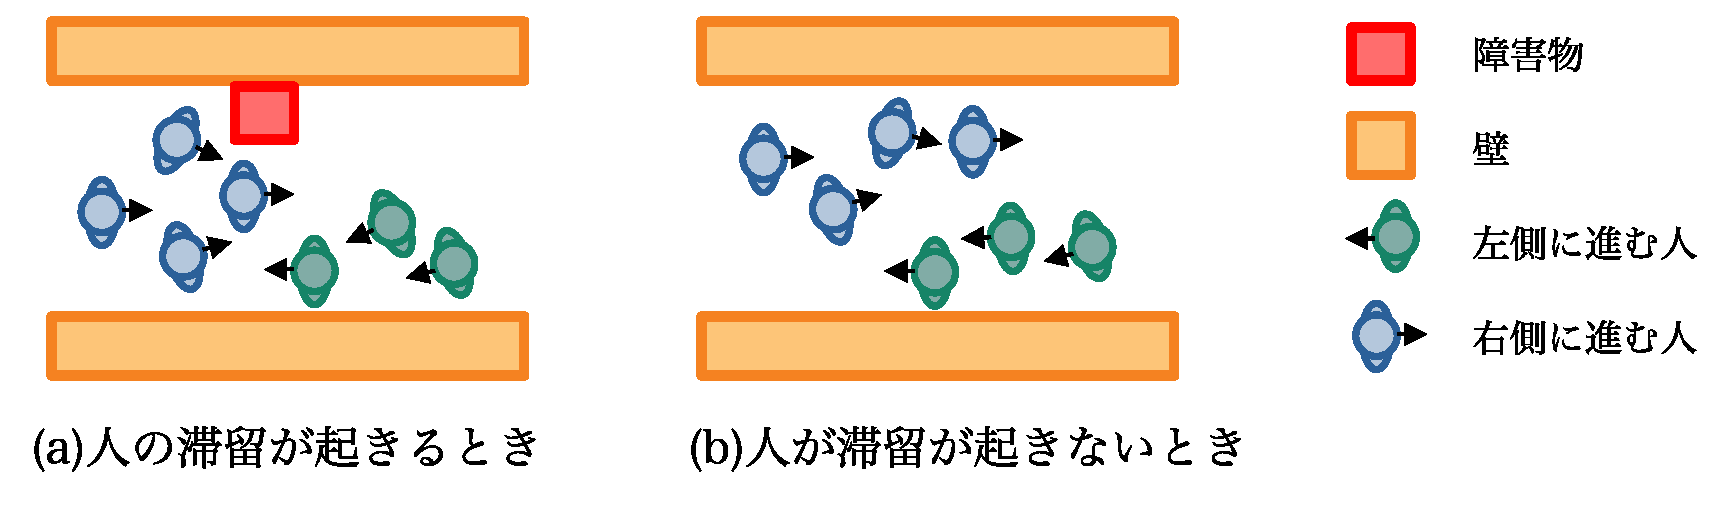
\includegraphics[width=14cm,clip]{figure/jinryu_image2_r2.eps}
     \caption{人流シミュレーションの活用例}
     \label{fig:jinryu_image}
    \end{center}
\end{figure}
%
%人流シミュレーションに必要な要素
人流シミュレーションを用いて人の動きを解析するためには,
人の動きを再現するための歩行者のモデル化(歩行者モデル)が必要である.
歩行者モデルは,求められる解析精度や解析規模に応じて使い分ける必要があるため,
ネットワークモデルやセルオートマトン,SocialForceModel(SFM)などが提案されている.
本章では,各歩行者モデルの使用用途や利点,欠点を用いて各手法の立ち位置について
述べる.

\section{歩行者モデル}
歩行者モデルは,歩行者の移動を決定するためのアルゴリズムである.
シミュレーション対象が海岸から近い都市や人口が多い都市などの道路上の人々の流れを解析するためには,
数千人から数万人の解析が可能なネットワークモデルが用いられる(参考文献).
また,シミュレーション対象が商業施設や駅構内などの施設上の人々を解析するためには,
フロアフィールドモデルやSFMが用いられる(参考文献).



\subsection{ネットワークモデルの歩行者モデル**}
ネットワークモデルは,人々の移動や行動をネットワーク構造としてモデル化する手法である.
図\ref{fig:network_ex}にネットワークモデルの例を示す.
%
\begin{figure}[h]
    \begin{center}
     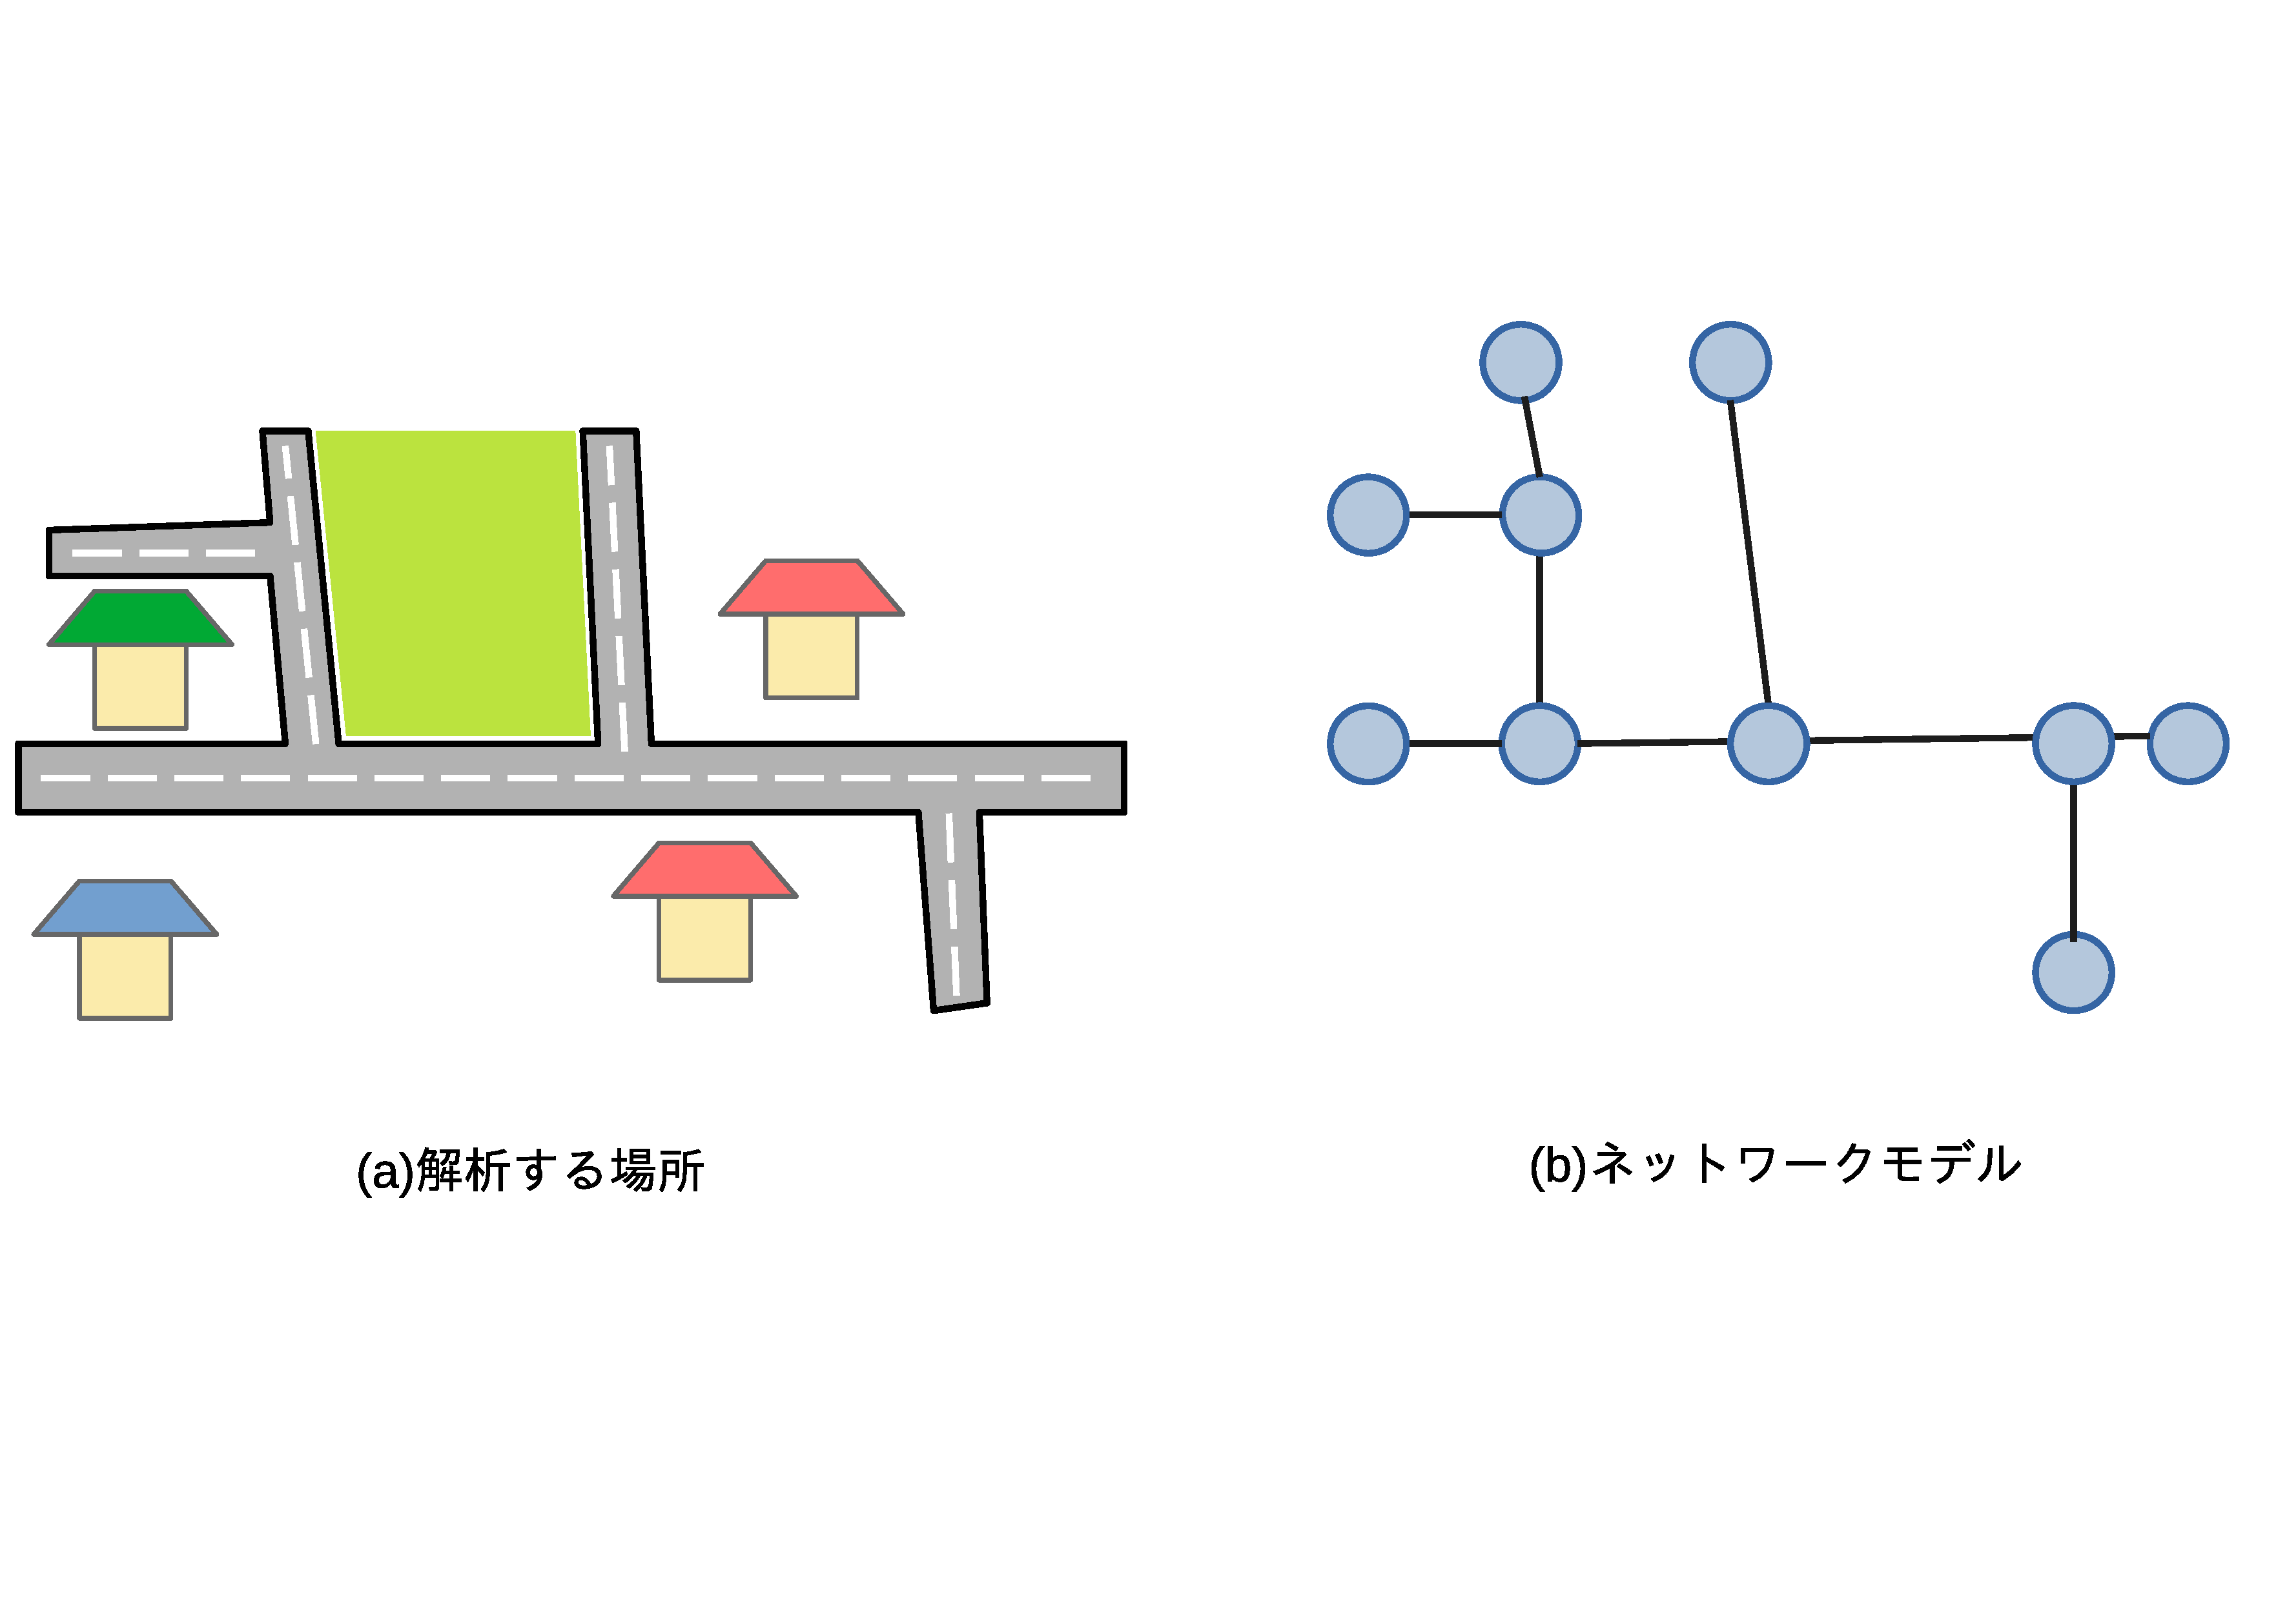
\includegraphics[width=14cm,clip]{figure/networkmodel_ex.eps}
     \caption{ネットワークモデルの例}
     \label{fig:network_ex}
    \end{center}
\end{figure}
%
図\ref{fig:network_ex}中の(a)は解析対象であり,(b)はネットワークモデルである.
図\ref{fig:network_ex}中の(b)の青丸は交差点や道路の末端であり,ノードと呼ばれる.
ネットワークモデルでは,ノード間に数十から数百人単位で動かすことで,人の動きを解析する.
ネットワークモデルは,解析が高速であるが,モデルの準備に大きな作業が必要になるだけでなく,
モデルの定義に知識や経験が必要になることが多い.
ネットワークモデルを用いた解析では,都市間の人々の移動や,津波や地震などの
災害時における都市の避難シミュレーションのような解析人数が多い解析に用いられることが多い
(参考文献)
ネットワークモデルで建物内の人の流れを解析する場合は,図\ref{fig:nework_situnai}に示すように
解析領域内にメッシュ状にノードを配置することで解析できる(参考文献).
一方で,建物内などの避難シミュレーションでは,人の流量が低下する原因や滞留の原因を調査する
ことに用いられることが多いため,ネットワークモデルを用いた場合は,滞留などの再現ができない.
このため,人の流量が低下する原因や滞留の原因を突き止めるために解析するときは,静的フロアモデルやSFM
などが用いられることが一般的である.


\subsection{静的フロアモデル}
静的フロアモデルは,図\ref{fig:serumaton}に示すようなフロアフィールドモデルの空間モデルを用いて
おり,格子ごとに目的地までの距離を設定し,確率を用いてエージェントを移動させることで解析する手法である.
図\ref{fig:huroa_model_image}に静的フロアフィールドモデルのイメージを示す.
図\ref{fig:huroa_model_image}中の格子は解析領域,青丸はエージェント,青色の矢印はエージェントの移動可能な
方向である.
図\ref{fig:huroa_model_image}のように,静的フロアフィールドモデルは,

\begin{figure}[t]
    \begin{center}
     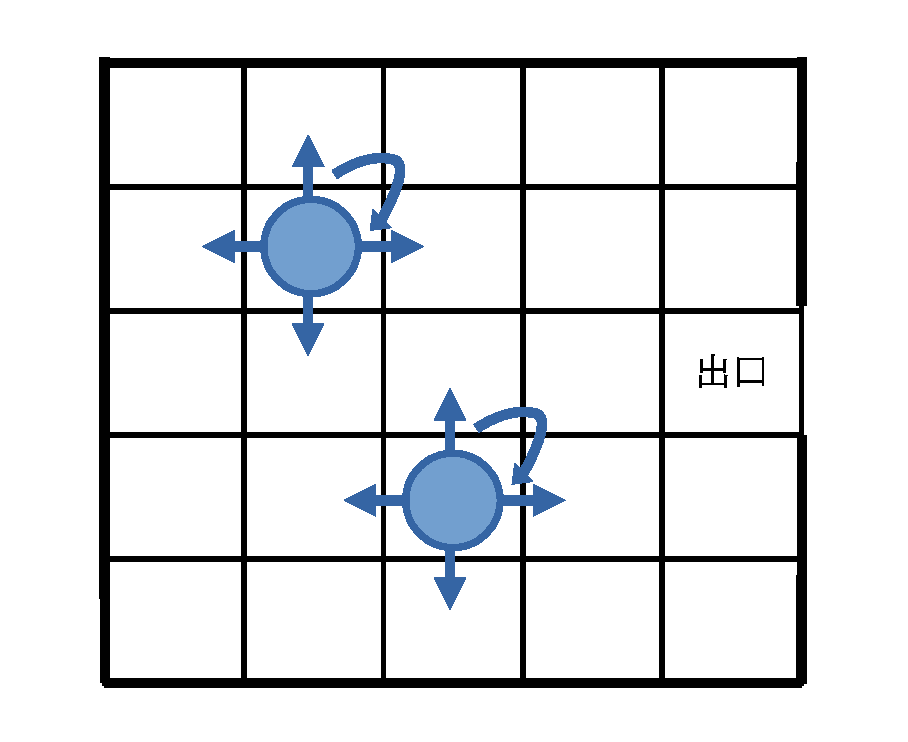
\includegraphics[width=7cm,clip]{figure/floormodel_image.eps}
     \caption{静的フロアフィールドモデルのイメージ}
     \label{fig:huroa_model_image}
    \end{center}
\end{figure}


図\ref{fig:huroa_model}に室内からの退出時における静的フロアフィールドの例を示す.
図\ref{fig:huroa_model}中の~~である.
図\ref{fig:huroa_model}中の(a)マンハッタン距離と(b)ユークリッド距離は,各格子から出口までの
距離を示す.

\begin{figure}[h]
    \begin{center}
     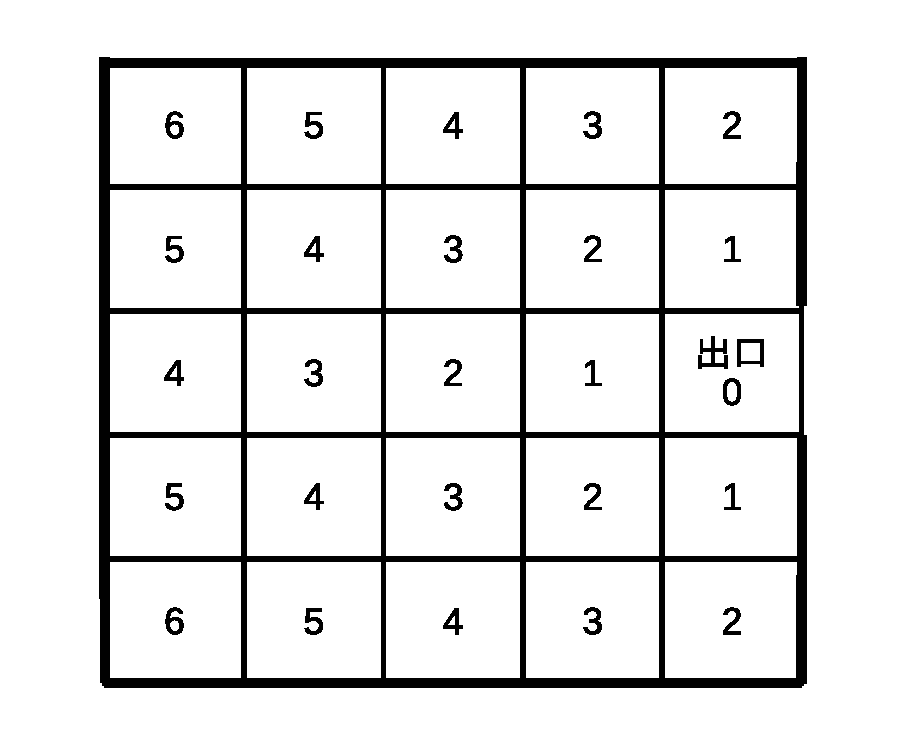
\includegraphics[width=7cm,clip]{figure/floormodel_kyori.eps}
     \caption{静的フロアフィールドモデルのイメージ}
     \label{fig:huroa_model_image}
    \end{center}
\end{figure}

\begin{figure}[h]
    \begin{center}
     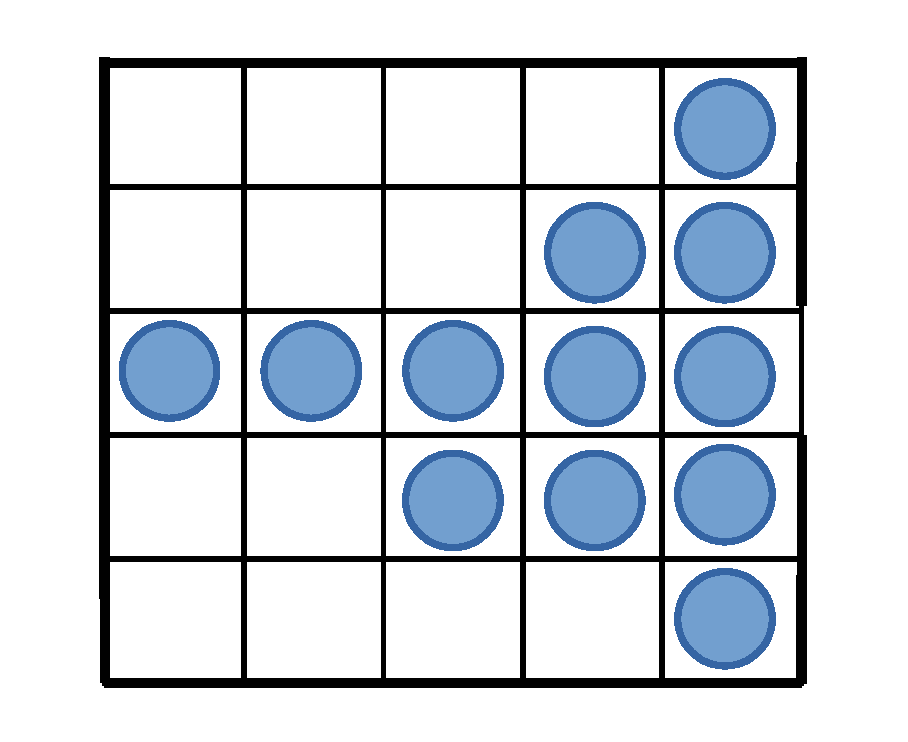
\includegraphics[width=7cm,clip]{figure/floormodel_ex2.eps}
     \caption{静的フロアフィールドモデルのイメージ}
     \label{fig:huroa_model_image}
    \end{center}
\end{figure}

静的フロアフィールドモデルは,計算対象のエージェントの周囲のセルのなかから,出口までの
距離が小さくなるようなセルを選択することで,出口までの解析が可能となる.
静的フロアフィールドモデルの利点は,解析前に各格子の計算を事前にできるため,非常に高速な
解析が可能である点である.
一方で,静的フロアフィールドは,出口前に形成されるアーチ現象の再現度が低いことが知られている.
図\ref{fig:huroa_model_ketten}に静的フロアフィールドモデルを用いた場合の出口前に形成される
アーチ現象の例を示す.
図\ref{fig:huroa_model_ketten}中の~~~である.
静的フロアフィールドモデルは,図\ref{fig;ruroa_model_ketten}のように,格子に一人のみ入ることができる
ことから,動きが格子サイズに制約されるため,出口付近の再現度が低い.
フロアフィールドモデルを用いた解析では,〇〇や△△,□□を用いることで,解析精度の向上が行われている
が,格子サイズの成約から,精度の向上に上限がある.
このため,高い解析精度が必要な場合は,SocialForceMoel(SFM)のような
解析領域を連続座標で解析する手法が用いられることが多い


\begin{figure}[htbp]
  \begin{minipage}[b]{0.5\linewidth}
    \centering
    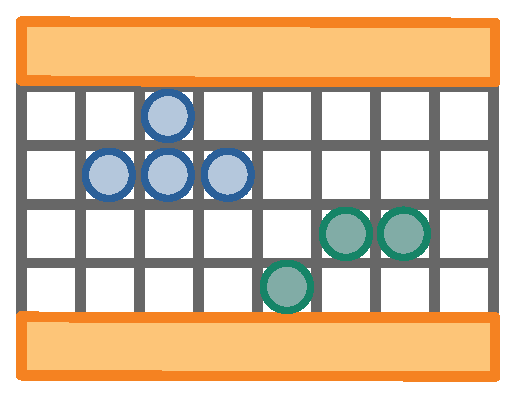
\includegraphics[keepaspectratio, scale=0.37]{figure/seruotomaton_image4.eps}
    \caption{フロアフィールドモデルの例}
    \label{fig:serumaton}
  \end{minipage}
  \begin{minipage}[b]{0.5\linewidth}
    \centering
    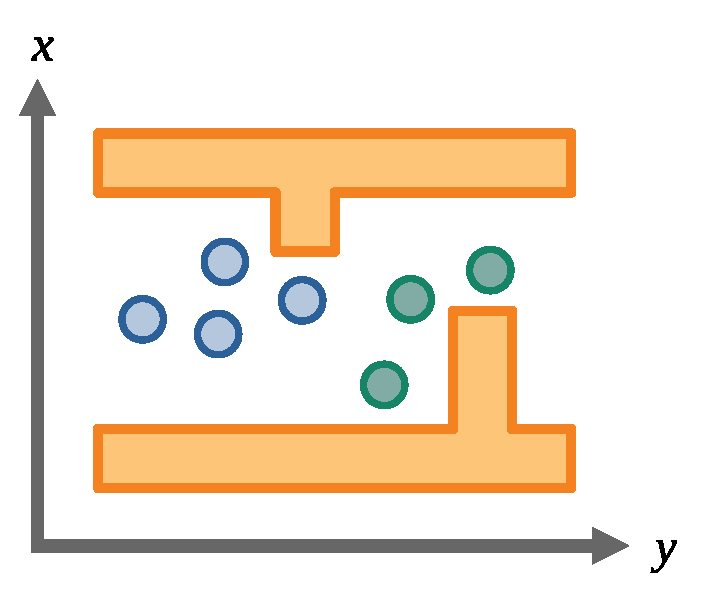
\includegraphics[keepaspectratio, scale=0.37]{figure/renzoku_image2.eps}
    \caption{二次元連続座標モデルの例}
    \label{fig:renzoku}
  \end{minipage}
\end{figure}



\subsection{SocialForceModel(SFM)}
SFMは,人間の社会心理学的な要素と物理的な力を結びつけた動力学モデルであり,
近傍のエージェントや壁といった障害物から受ける力によってエージェントの進行方向
や速度を解く.本手法は,心理的変数が組み込まれているため,災害時の避難シミュ
レーションによく用いられる\cite{21_Isozaki}\cite{ando_sfm}.

%\section{仮)SFMの解析空間}
SFMの解析空間は,二次元
連続空間モデルが用いられる.二次元連続空間モデルは,解析領域を分割せずに$(x,y)$の連続した座標で
解析する手法である.図\ref{fig:renzoku}に図\ref{fig:jinryu_image2}の例を二次元連続座標で
考えた例を示す.図\ref{fig:renzoku}中の矢印は座標の$x$と$y$を示している.SFMは,
図\ref{fig:serumaton}のフロアフィールドモデルのように格子上のエージェント数に制限がなく,
エージェントの位置を座標で考えるため,人流の再現度が高い.
%\section{仮)SFMにおけるエージェント移動}
SFMにおけるエージェント移動は,目的地へ進む力と他のエージェントから受ける力,
壁などの障害物から受ける力を用いる運動方程式を用いて求める.
式(\ref{eq:sfm_siki1})にSFMの運動方程式を示す.
%
\begin{eqnarray}
 m_i \frac{dv_i}{dt} = m_i \frac{v_i^0(t)e_i^0(t)-v_i(t)}{t_i}
 +\sum_{j(\neq i)}f_{ij}+\sum_{W}f_{iW}
 \label{eq:sfm_siki1}
\end{eqnarray}
%
式(\ref{eq:sfm_siki1})中の
総和の記号$\sum_{j(\neq i)}f_{ij}$は,エージェント$i$以外のすべ
てのエージェント$j$の総和をとることを意味する.同様に,$\sum_{W}f_{iW}$
は,すべての壁$W$の総和をとることを意味する.式
(\ref{eq:sfm_siki1})中の$m_i$はエージェント$i$の体重,$v_i^0(t)$はエージェ
ントの希望速度,$e_i^0(t)$は,目的地までの単位ベクトル,$v_i(t)$
は現在の速度ベクトル,$t_i$は時定数である.式(\ref{eq:sfm_siki1})の第一
項はエージェントが目的地へ進む力,第二項は他のエージェントから受ける力
$f_{ij}$,第三項は壁などの障害物から受ける力$f_{iW}$の合力である.
$f_{ij}$と$f_{iW}$は,式(\ref{eq:sfm_siki2})と式(\ref{eq:sfm_siki3})を用
いて導出する.
%
\begin{eqnarray}
 f_{ij} = & \{A_i exp[\frac{r_{ij} - d_{ij}}{B_i}]
  + kg(r_{ij} - d_{ij})\} n_{ij}
+ \kappa g (r_{ij} - d_{ij}) \Delta
  v^t_{ij} t_{ij}
 \label{eq:sfm_siki2}
\end{eqnarray}
%
\begin{eqnarray}
 f_{iW} = \{A_i exp[\frac{r_{i} - d_{iW}}{B_i}]
  + kg(r_{i} - d_{iW})\} n_{iW} + \kappa g (r_{i} - d_{iW})
  (v_i t_{iW}) t_{iW}
 \label{eq:sfm_siki3}
\end{eqnarray}
%
表\ref{tab:tab_para}に
式(\ref{eq:sfm_siki2}),(\ref{eq:sfm_siki3})中の変数を示す.
衝突時関数$g(x)$はエージェント同士や壁などに衝突したときに値をとる関数
である.式(\ref{eq:gx_siki})に衝突時関数$g(x)$の条件式を示す.
%
\begin{equation}
  \label{eq:gx_siki}
  g(x) =
  \begin{cases}
    1 & (x<0) \\
    0 & otherwise
  \end{cases}
\end{equation}
%
SFMの衝突時の計算は,条件式である式(\ref{eq:gx_siki})を用いることで,衝突時のみ計算できる.
SFMを用いる人流シミュレーションのフローチャートを図
\ref{fig:sfm_flowchart}に示す.
図\ref{fig:sfm_flowchart} 中の目的地へ進む力の計算は,式(\ref{eq:sfm_siki1})中の第一項を
用いて算出する.また,他のエージェントから受ける力の計算は,式(\ref{eq:sfm_siki2})を用いて
算出する.そして,壁などの障害物から受ける力の計算は,式(\ref{eq:sfm_siki3})を用いて算出する.
SFMを用いた人流シミュレーションは,図\ref{fig:sfm_flowchart}に示すように,
式(\ref{eq:sfm_siki1})の運動方程式を積分することで,新しい時間のエージェントの位置と速度を求
めることができる.


\begin{table}[hbtp]
 \begin{center}
  \caption{SFMのパラメータ}
    \begin{tabular}{c|c}
     \hline \hline
     $d_{ij}$ & エージェント間の距離 \\
     \hline
     $t_{ij}$ & エージェント$i$とエージェント$j$の衝突面の垂直ベクトル \\
     \hline
     $n_{ij}$ & エージェント$i$とエージェント$j$の衝突面の法線ベクトル\\
     \hline
     $r_i$ & エージェント$i$の体の半径 \\
     \hline
     $r_{ij}$ & エージェント$i$とエージェント$j$の体の半径の和 \\
     \hline
     $t_{iW}$ & エージェント$i$と壁$W$の衝突面の垂直ベクトル\\
     \hline
     $n_{iW}$ & エージェント$i$とエージェント$W$の衝突面の法線ベクトル \\
     \hline
     $A_i$ & エージェント$i$のインタラクション作用 \\
     \hline
     $B_i$ & エージェント$i$の反発作用 \\
     \hline
     $k$ & 衝突時の反発力係数\\
     \hline
     $\kappa$ & 衝突時の摩擦力係数 \\
     \hline
     $\Delta v_{ij}$ & エージェント$i$とエージェント$j$の接線速度の差 \\
     \hline
     $g(x)$ & 衝突時関数 \\
     \hline
    \end{tabular}
  \label{tab:tab_para}
 \end{center}
\end{table}

\begin{figure}[hbtp]
 \begin{center}
  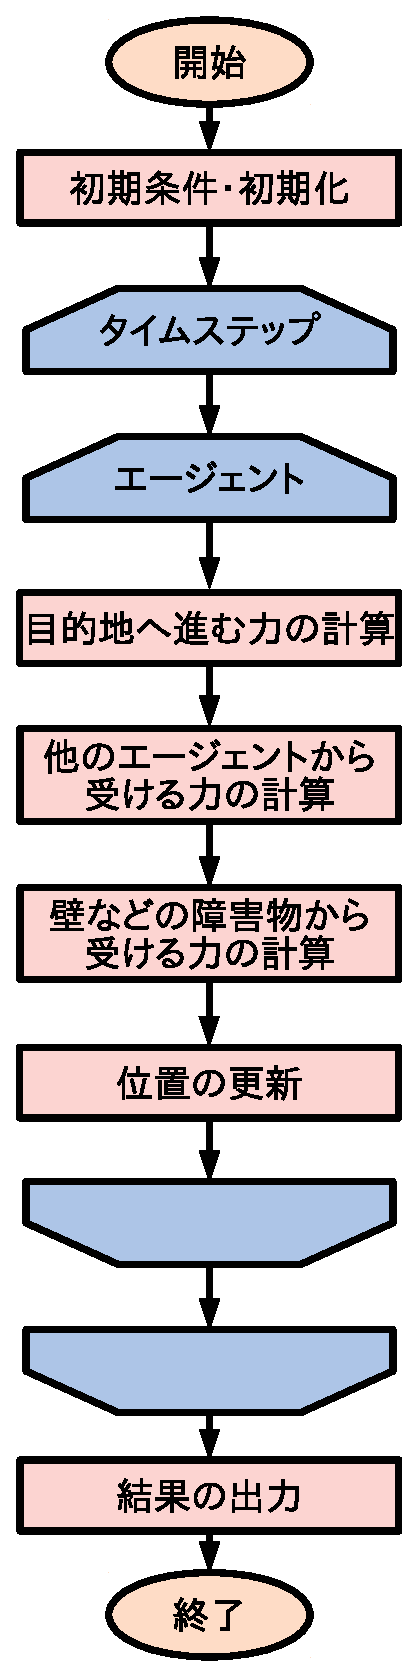
\includegraphics[width=4cm,clip]{figure/sfm_flowchart.eps}
  \caption{SFMを用いた人流シミュレーションのフローチャート}
  \label{fig:sfm_flowchart}
 \end{center}
\end{figure}

\begin{figure}[hbtp]
 \begin{center}
  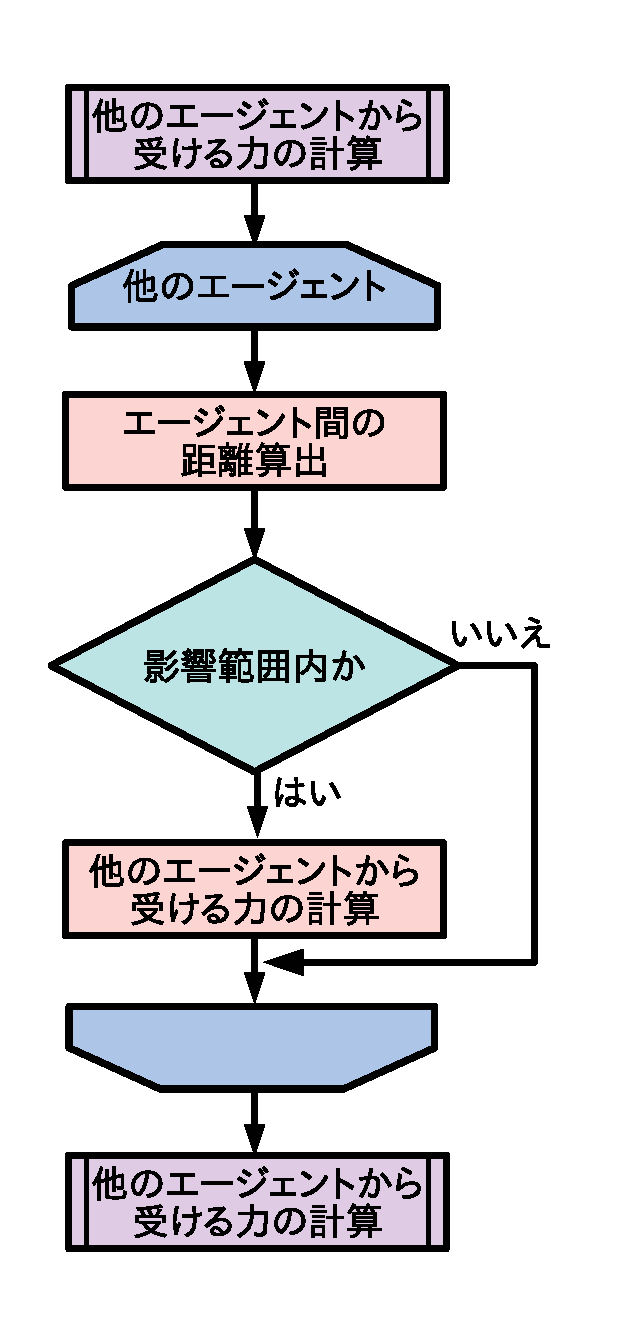
\includegraphics[width=4cm,clip]{figure/agent_flow.eps}
  \caption{SFMにおける周囲のエージェントから受ける力の計算}
  \label{fig:sfm_flowchart}
 \end{center}
\end{figure}

\begin{figure}[hbtp]
 \begin{center}
  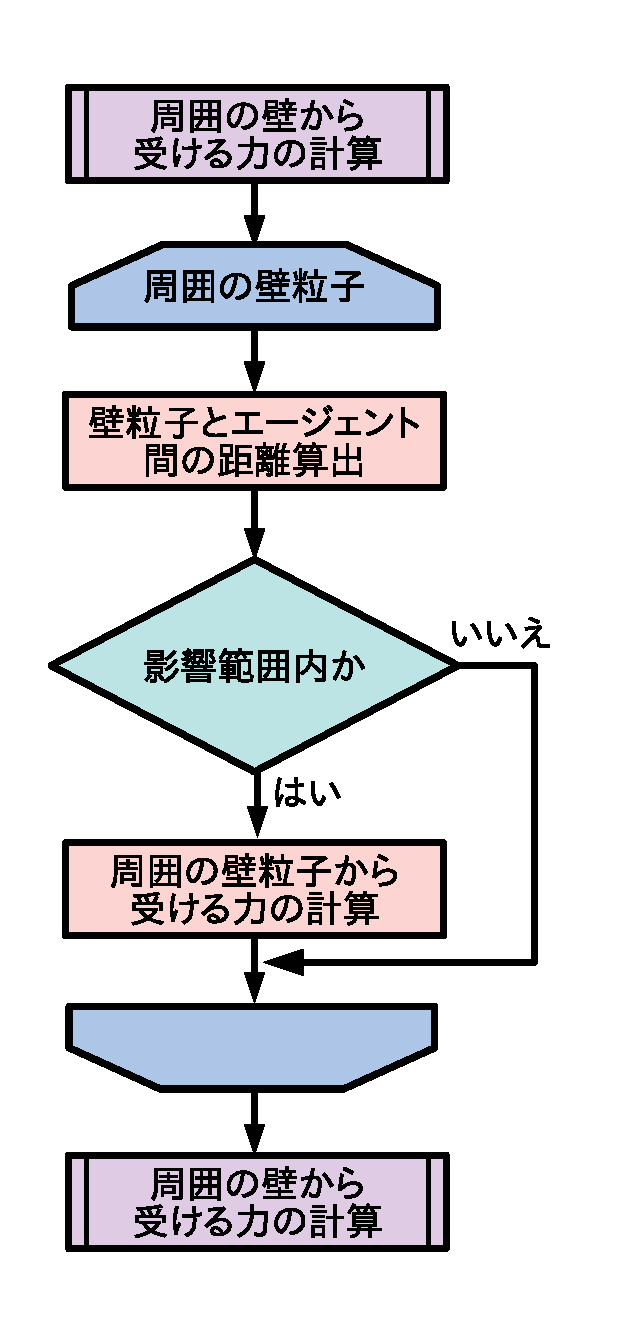
\includegraphics[width=4cm,clip]{figure/kabe_flow.eps}
  \caption{SFMにおける周囲の壁から受ける力の計算}
  \label{fig:sfm_flowchart}
 \end{center}
\end{figure}

他のエージェントから受ける力は,解析領域全体に存在する他のエージェントから
受ける.このため,SFMは,解析する人数が増えると他のエージェントから受ける
力の計算時間が長くなる.他のエージェントから受
ける力の計算負荷を削減するために,SFMを用いる人流シミュレーションでは,
他のエージェントから受ける力を計算する範囲を限定することが多い
\cite{seru_sfm1}\cite{seru_sfm2}.
他のエージェントから受ける力を計算する範囲を限定することで,遠くに存在する
エージェントから受ける力を0に近似することができる.
図\ref{fig:sougo_hani}に他のエージェントから受ける力の計算範囲の例
を示す.図\ref{fig:sougo_hani}の赤丸は他のエージェントから受ける力を計算
するエージェント,黒丸はエージェント4が計算するときの他のエージェント,
オレンジ色の点線は他のエージェント
から受ける力の範囲を示す.図\ref{fig:sougo_hani} のエージェント4は,
オレンジ色の点線内に存在するエージェント0,1,2,6,7,10の合計5人から力を
受ける.本論文では,近くのエージェントから受ける力の範囲を限定するSFMを前提
として述べる.
近くのエージェントから受ける力の範囲は,図\ref{fig:sougo_hani}の
ように,計算するエージェントの半径数メートルの範囲である.このため,SFMでは,
他のエージェントが近くのエージェントから受ける力の範囲に存在するか判定が必要
である.
この範囲に存在するかの判定は,エージェント$i$とエージェント$j$とのエージェン
ト間の距離$d_{ij}$の算出が必要である.
本論文では,式(\ref{eq:kyori_siki})を用いてエージェント間の距離$d_{ij}$
を求め,他のエージェントから受ける力の範囲内であるかどうか判定する.

\begin{eqnarray}
 d_{ij} =  \sqrt{ (x_i-x_j)^2 + (y_i-y_j)^2 }
 \label{eq:kyori_siki}
\end{eqnarray}

式(\ref{eq:kyori_siki})中の$x_i$と$y_i$はエージェント$i$の座標$(x_i,y_i)$,$x_j$
と$y_j$はエージェント$j$の座標$(x_j,y_j)$である.エージェント$i$は
,式(\ref{eq:kyori_siki})
で求めたエージェント距離$d_ij$が他のエージェントから受ける力の範囲内であれば,
エージェント$j$から式(\ref{eq:sfm_siki2})を用いて算出した力を受ける.
他のエージェントから受ける力の範囲の半径を$R$としたとき,エージェント$i$の他のエージェント
$j$が範囲内にいるかどうかの判定式を式(\ref{eq:jouken_siki1})に示す.

\begin{eqnarray}
  \label{eq:jouken_siki1}
  R \geq d_{ij}
\end{eqnarray}

エージェント$i$は,式(\ref{eq:jouken_siki1})の条件を満たす他のエージェント$j$から式(\ref{eq:sfm_siki2})
で求まる力を受ける.

他のエージェントから受ける力の範囲を限定するSFMのフローチャート
を図\ref{fig:sougosayou_flow}に示す.
図\ref{fig:sougosayou_flow}のフローチャートでは,各エージェントに対しエー
ジェント間の距離を計算し,範囲内であるか判定することで,他のエージェントから受ける力の範囲を限定
している.SFMを用いる人流シミュレーションは,他のエージェントから受ける力の範囲を視野の範囲に
することで,視野を再現できる.

\begin{figure}[hbtp]
 \begin{center}
  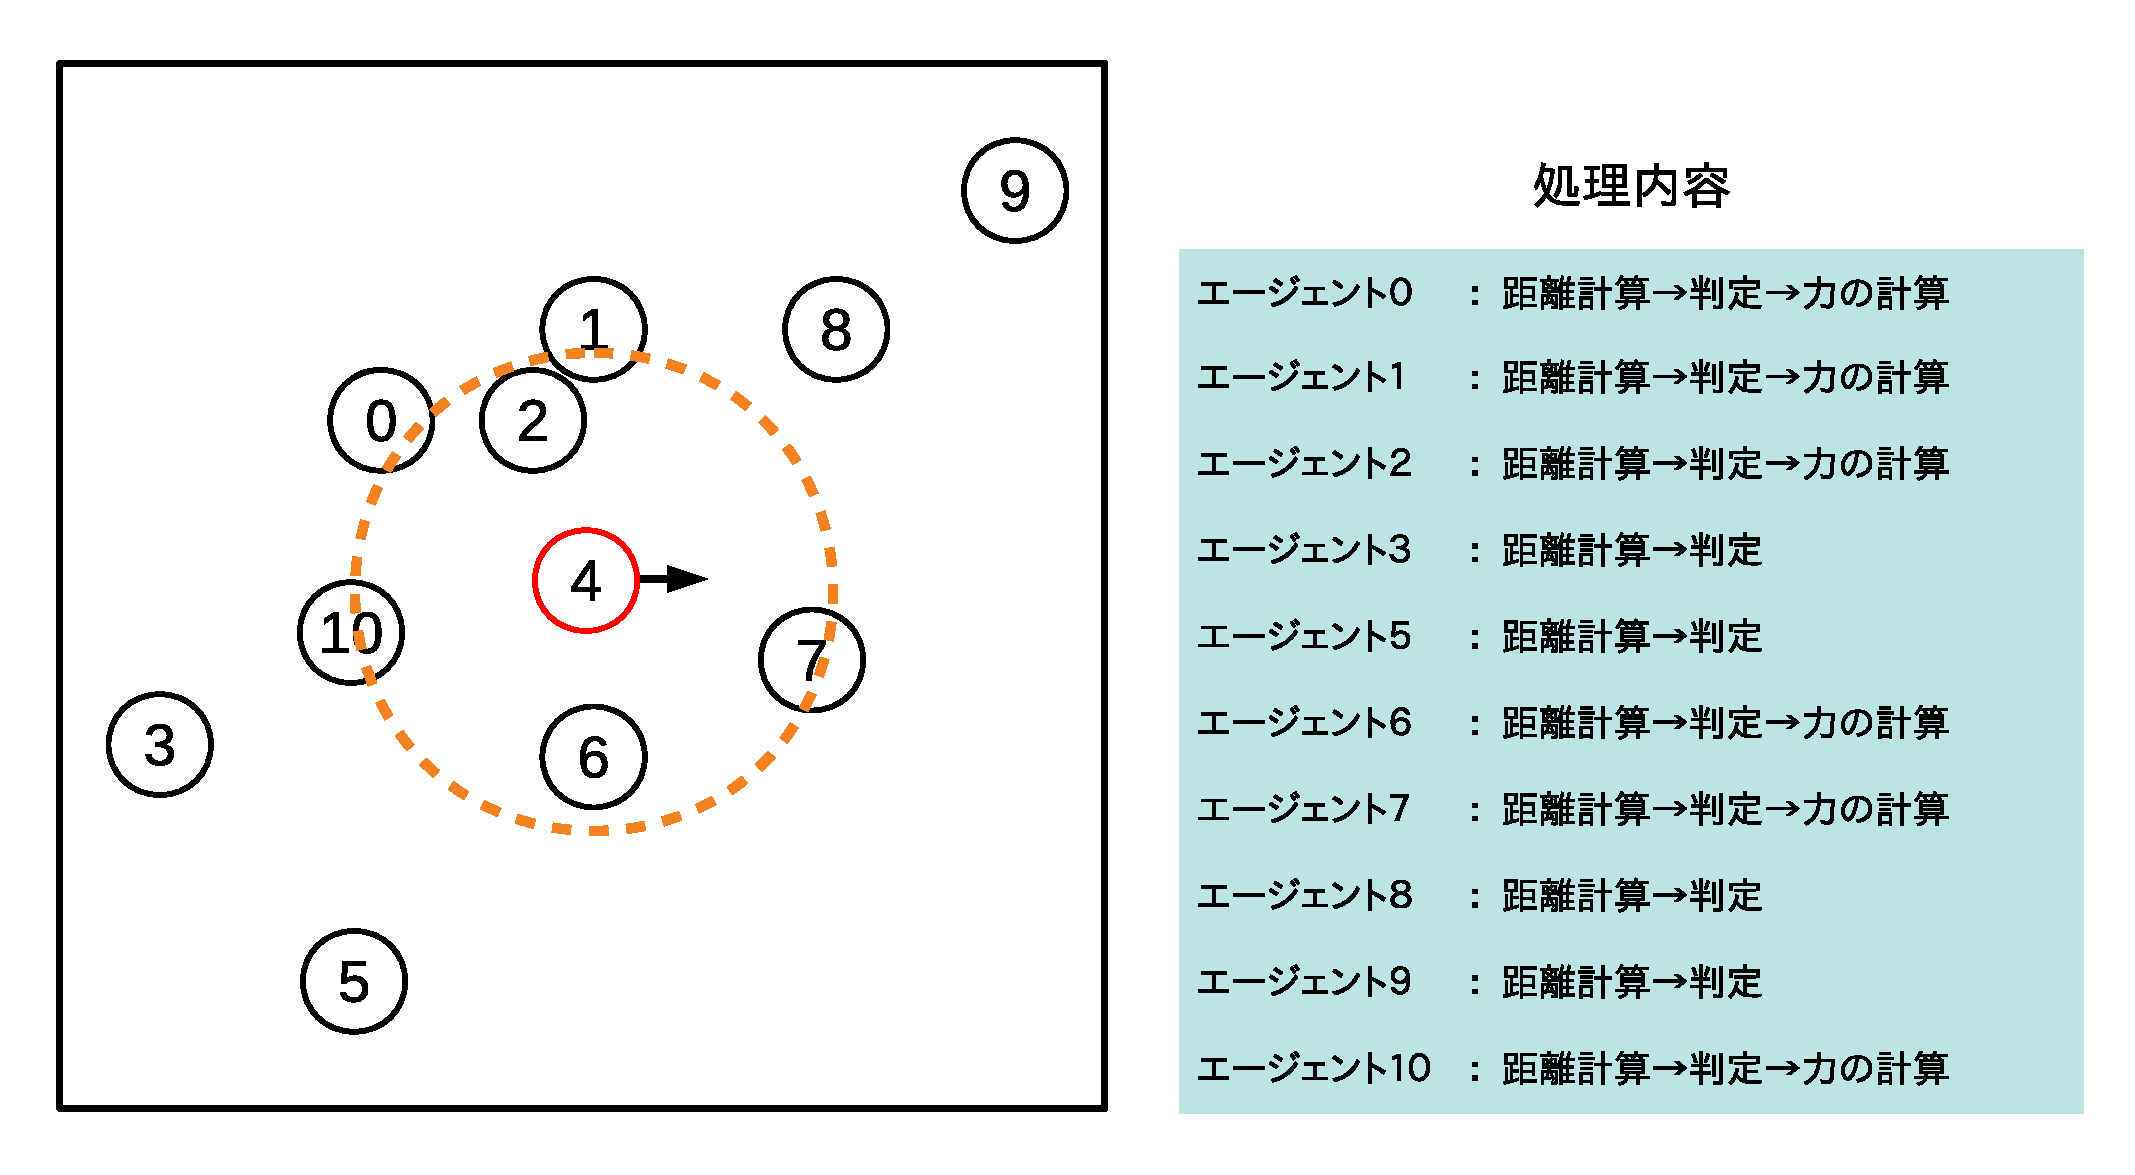
\includegraphics[width=11.5cm,clip]{figure/sougo_hani_image_r2.eps}
  \caption{他のエージェントから受ける力の範囲を限定するときの例}
  \label{fig:sougo_hani}
 \end{center}
\end{figure}

%経由地のことを述べる


\begin{figure}[hbtp]
 \begin{center}
  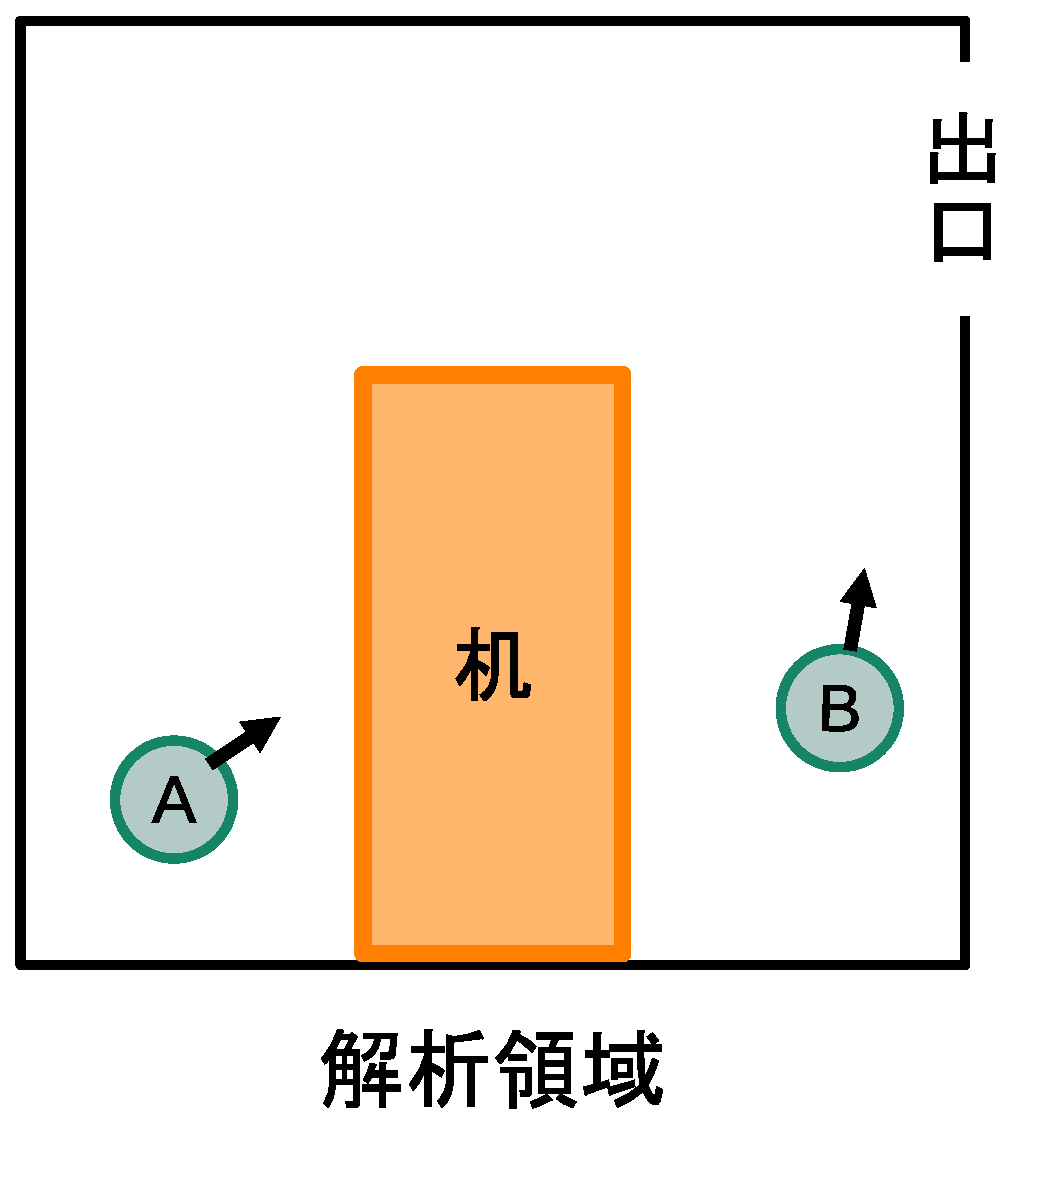
\includegraphics[height=4cm,clip]{figure/sutakku_ex.eps}
  \caption{SFMでスタック現象が起きる例}
  \label{fig:sougo_hani}
 \end{center}
\end{figure}

\begin{figure}[hbtp]
 \begin{center}
  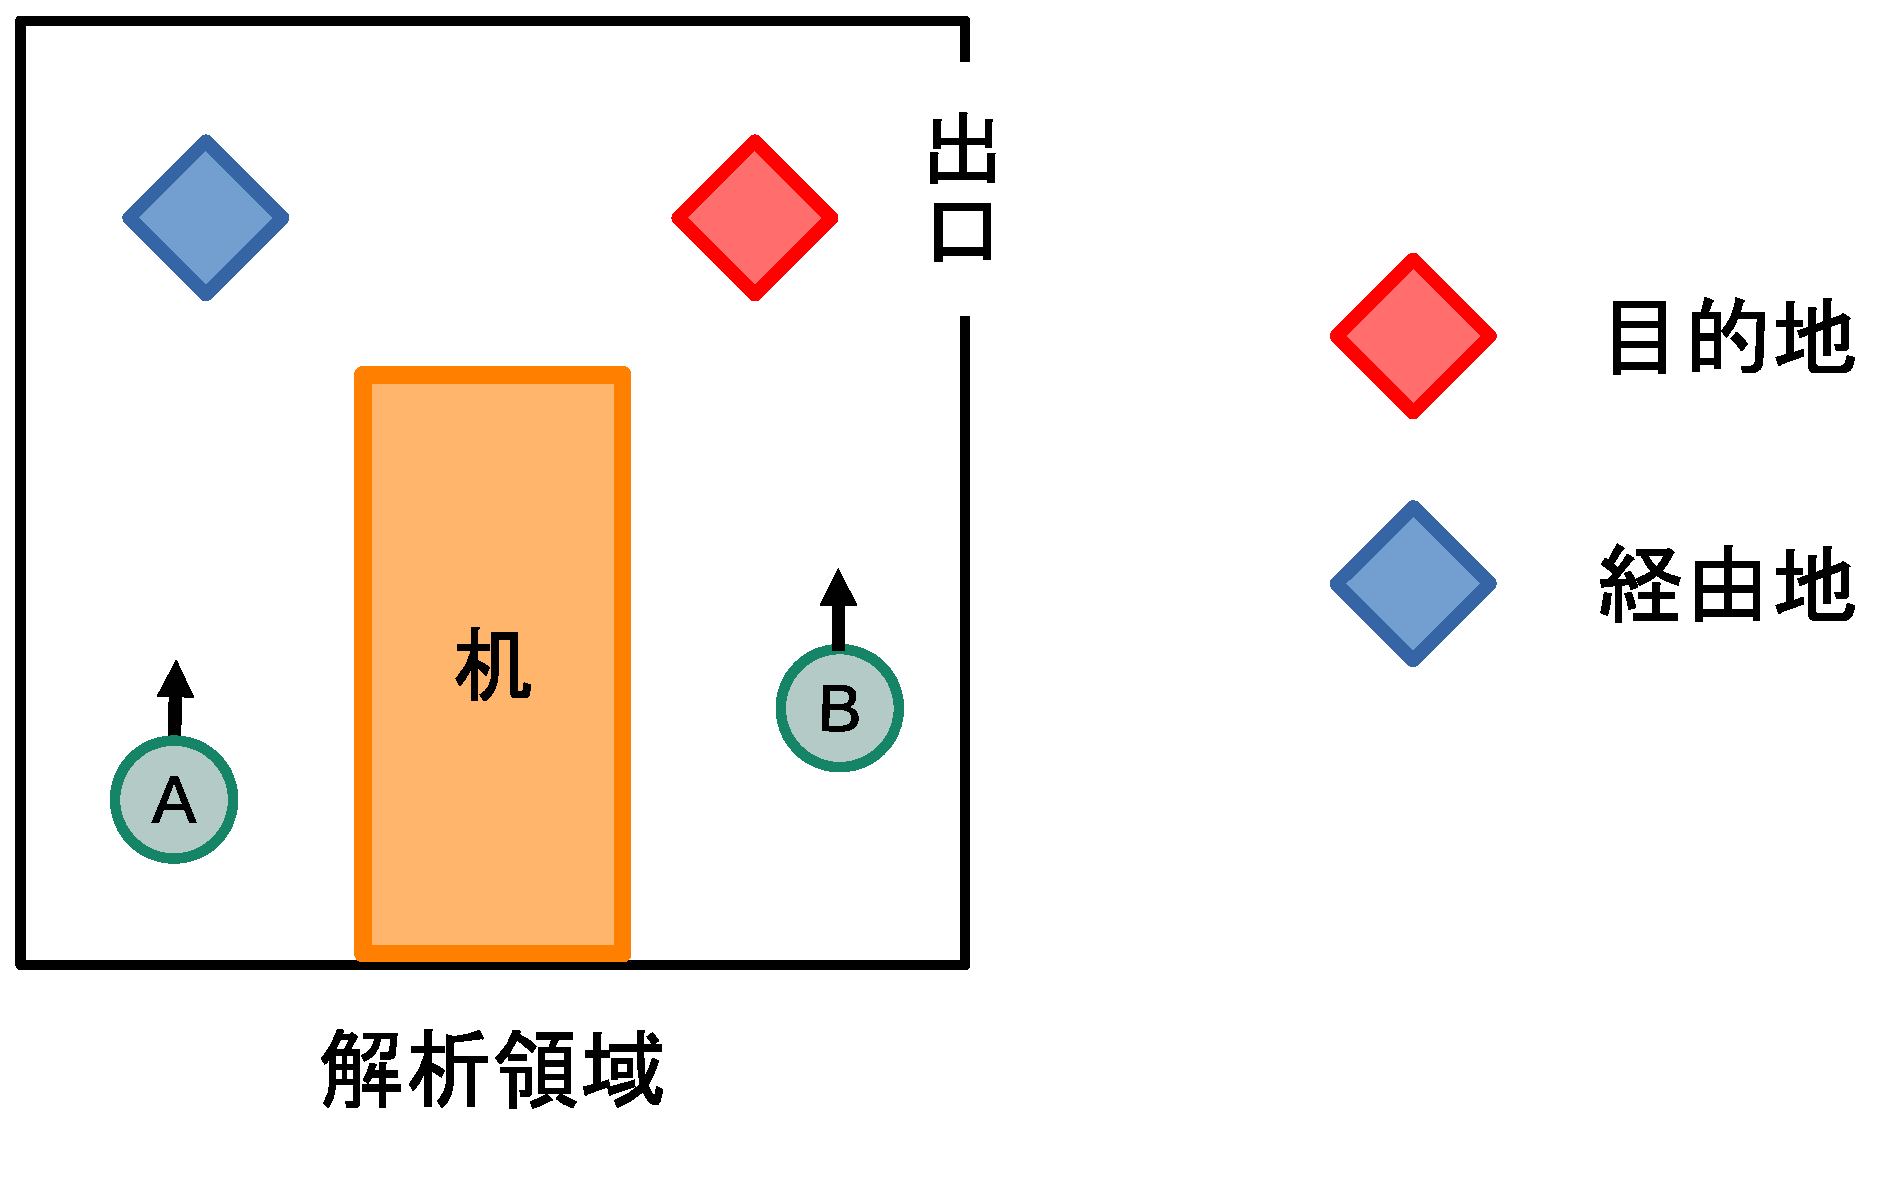
\includegraphics[height=4cm,clip]{figure/keiyuti_ex.eps}
  \caption{経由地を設定するSFMの例}
  \label{fig:sougo_hani}
 \end{center}
\end{figure}

\begin{figure}[hbtp]
 \begin{center}
  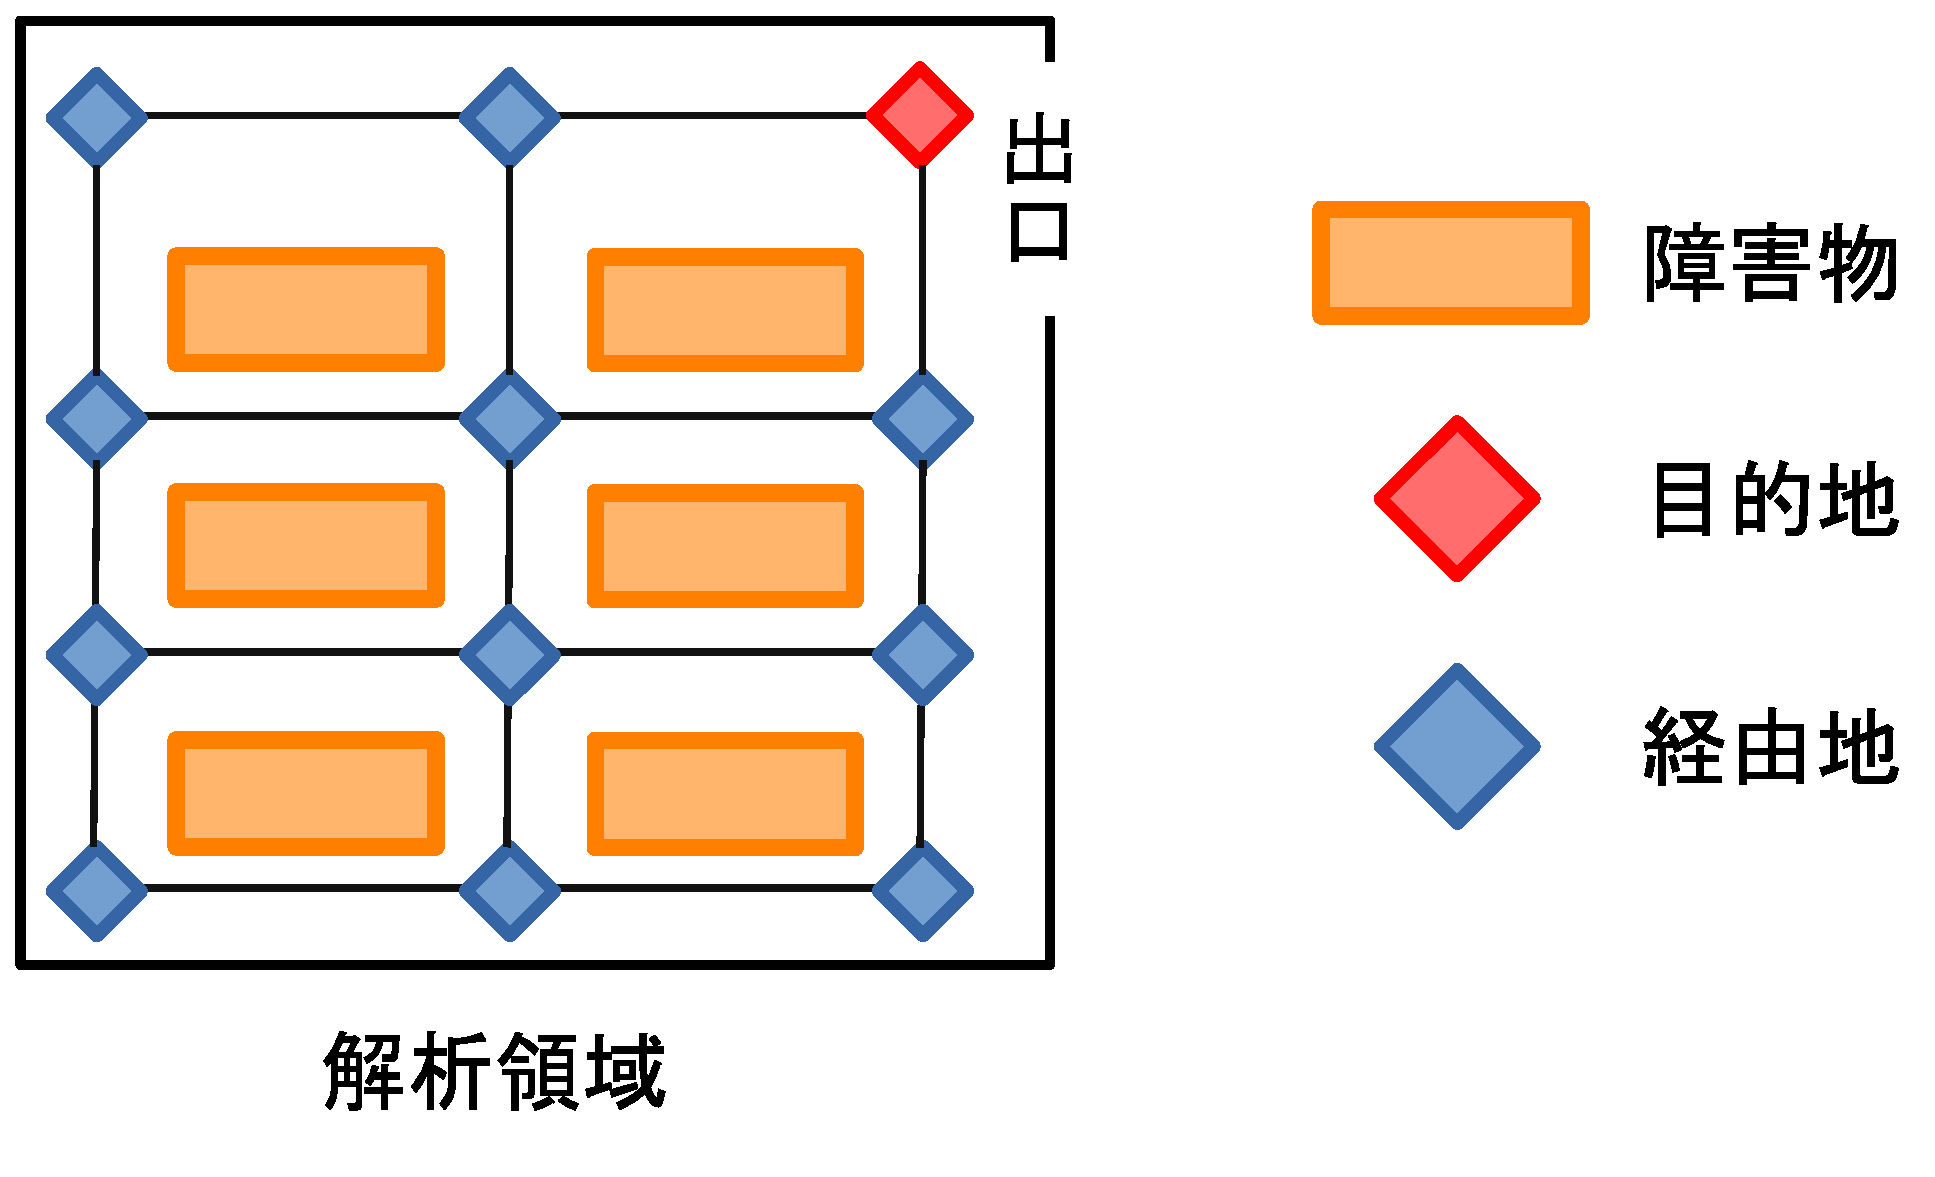
\includegraphics[height=4cm,clip]{figure/keiyuti_ex2.eps}
  \caption{経由地を設定するSFMの例}
  \label{fig:sougo_hani}
 \end{center}
\end{figure}



%論文引用{{{
\if 0
SFMは,人間の社会心理学的な要素と物理的な力を結びつけた物力学モデルであり,
周囲のエージェントや壁や机などの障害物から受ける力を用いてエージェントの
進行方向や速度を決定する.
人間の社会心理学的な要素は,周囲に人がいるときに避けようとする人間の心理を
利用したものである.物理学的な力は,人と人や人と障害物が衝突したときに生じる
力である.
本手法は,心理的変数が組み込まれているため,災害時の避難シミュレーションによく
用いられる(参考文献[卒論を参照])
SFMの解析空間は,二次元の連続空間モデルが用いられる.



SocialFroceModel(SFM)は,周囲の状況に基づいて生成した運動方程式を用いて時間ステップ$t$ごとに
エージェントの移動を決定する.
\eq{sfm_siki1}にエージェント$i$の運動方程式を示す.
%
\begin{eqnarray}
  m_i \frac{dv_i}{dt} = m_i \frac{v_i^0 e_i - v_i}{\tau_i}
  +\sum_{j(\neq i)}f_{ij}+\sum_{W}f_{iW}
  \label{eq:sfm_siki1}
\end{eqnarray}
%
\eq{sfm_siki1}中の
右辺第一項はエージェントが目的地へ進む力を表しており,
エージェント$i$の体重$m_i$,
希望速度$v_i^0$,
目的地までの単位ベクトル$e_i$,現在の速度ベクトル$v_i$,
時定数$\tau_i$に基づいて算出される.
右辺第二項は周囲のエージェントを避ける力であり,
$f_{ij}$はエージェント$i$とエージェント$j$の相互作用力である.
また,第三項は壁などの障害物を避ける力であり,
$f_{iW}$はエージェント$i$が壁などの障害物$W$から受ける力である.
$f_{ij}$や$f_{iW}$は,\eq{sfm_siki2}と\eq{sfm_siki3}から算出する.
%
\begin{eqnarray}
  f_{ij} =  \{A_i exp [\frac{r_{ij} - d_{ij}}{B_i}  ]
  + kg(r_{ij} - d_{ij})\} n_{ij} \\ \nonumber
  + \kappa g (r_{ij} - d_{ij}) \Delta
  v^t_{ij} t_{ij}
  \label{eq:sfm_siki2}
\end{eqnarray}
%
\begin{eqnarray}
  f_{iW} = \{A_i exp[\frac{r_{i} - d_{iW}}{B_i}]
  + kg(r_{i} - d_{iW})\} n_{iW} \\ \nonumber
  + \kappa g (r_{i} - d_{iW}) (v_i t_{iW}) t_{iW}
  \label{eq:sfm_siki3}
\end{eqnarray}
%
式中の$r_i$はエージェント$i$の体の半径,
$t_{iW}$はエージェント$i$と壁$W$の垂直ベクトル,
$n_{iW}$はエージェント$i$と壁$W$の衝突面の法線ベクトル,
$A_i$はエージェント$i$のインタラクション作用,
$B_i$はエージェント$i$の反発作用,
$k$は衝突時の反発力係数,
$\kappa$は衝突時の摩擦力係数
である.
$d_{ij}, t_{ij}, n_{ij}, r_{ij}, \Delta v_{ij}$は,
エージェント$i$,$j$間の距離,
衝突面の垂直ベクトル,衝突面の法線ベクトル,体の半径の和,接線速度の差である.
また,衝突時関数$g(x)$は,\eq{gx_siki}に示すように$x$に応じてエージェント同士
の衝突を判定する.
%
\begin{equation}
  \label{eq:gx_siki}
  g(x) =
  \begin{cases}
    1 & (x<0)     \\
    0 & otherwise
  \end{cases}
\end{equation}
%
衝突時関数$g(x)$中の$x$は,エージェント同士の距離やエージェントと壁の距離であり,
衝突時であれば1,衝突していなければ0となる.
\fi
%}}}


\section{障害物モデル}

\subsection{粒子によるモデル化}

\subsection{矩形によるモデル化}

\section{経路の設定}

\subsection{ダイクストラ法}



%1ブロックが10×30文字です
ああああああああああああああああああああああああああああああ
ああああああああああああああああああああああああああああああ
ああああああああああああああああああああああああああああああ
ああああああああああああああああああああああああああああああ
ああああああああああああああああああああああああああああああ
ああああああああああああああああああああああああああああああ
ああああああああああああああああああああああああああああああ
ああああああああああああああああああああああああああああああ
ああああああああああああああああああああああああああああああ
ああああああああああああああああああああああああああああああ
%
ああああああああああああああああああああああああああああああ
ああああああああああああああああああああああああああああああ
ああああああああああああああああああああああああああああああ
ああああああああああああああああああああああああああああああ
ああああああああああああああああああああああああああああああ
ああああああああああああああああああああああああああああああ
ああああああああああああああああああああああああああああああ
ああああああああああああああああああああああああああああああ
ああああああああああああああああああああああああああああああ
ああああああああああああああああああああああああああああああ
%
Penguin
ああああああああああああああああああああああああああああああ
ああああああああああああああああああああああああああああああ
ああああああああああああああああああああああああああああああ
ああああああああああああああああああああああああああああああ
ああああああああああああああああああああああああああああああ
ああああああああああああああああああああああああああああああ
ああああああああああああああああああああああああああああああ
ああああああああああああああああああああああああああああああ
ああああああああああああああああああああああああああああああ
ああああああああああああああああああああああああああああああ
%
ああああああああああああああああああああああああああああああ
ああああああああああああああああああああああああああああああ
ああああああああああああああああああああああああああああああ
ああああああああああああああああああああああああああああああ
ああああああああああああああああああああああああああああああ
ああああああああああああああああああああああああああああああ
ああああああああああああああああああああああああああああああ
ああああああああああああああああああああああああああああああ
ああああああああああああああああああああああああああああああ
ああああああああああああああああああああああああああああああ
%
ああああああああああああああああああああああああああああああ
ああああああああああああああああああああああああああああああ
ああああああああああああああああああああああああああああああ
ああああああああああああああああああああああああああああああ
ああああああああああああああああああああああああああああああ
ああああああああああああああああああああああああああああああ
ああああああああああああああああああああああああああああああ
ああああああああああああああああああああああああああああああ
ああああああああああああああああああああああああああああああ
ああああああああああああああああああああああああああああああ
ああああああああああああああああああああああああああああああ
%
ああああああああああああああああああああああああああああああ
ああああああああああああああああああああああああああああああ
ああああああああああああああああああああああああああああああ
ああああああああああああああああああああああああああああああ
ああああああああああああああああああああああああああああああ
ああああああああああああああああああああああああああああああ
ああああああああああああああああああああああああああああああ
ああああああああああああああああああああああああああああああ
ああああああああああああああああああああああああああああああ
%
ああああああああああああああああああああああああああああああ
ああああああああああああああああああああああああああああああ
ああああああああああああああああああああああああああああああ
ああああああああああああああああああああああああああああああ
ああああああああああああああああああああああああああああああ
ああああああああああああああああああああああああああああああ
ああああああああああああああああああああああああああああああ
ああああああああああああああああああああああああああああああ
ああああああああああああああああああああああああああああああ
ああああああああああああああああああああああああああああああ
%
ああああああああああああああああああああああああああああああ
ああああああああああああああああああああああああああああああ
ああああああああああああああああああああああああああああああ
ああああああああああああああああああああああああああああああ
ああああああああああああああああああああああああああああああ
あああああああああああああああああああああ
あああああああああああああああああああああ
%
%\chapter{背景(1671文字)}

%***** END ************************************************
